% !TeX spellcheck = en_US

\documentclass[
	11pt,
	a4paper,
	usegeometry,
	twoside,
	openright,
	toc=chapterentrywithdots
]{scrbook}

\KOMAoptions{
	listof=totoc,
	bibliography=totoc,
	index=totoc
}

\usepackage[T1]{fontenc}
\usepackage[utf8]{inputenc}
\usepackage[ngerman,english]{babel}
\usepackage[english]{datetime2}

\usepackage{libertine}
%\usepackage[sc]{mathpazo}
% Maybe this for math: \usepackage{libertinust1math}
%\usepackage{courier}
%\usepackage{inconsolata}
%\renewcommand*\ttdefault{cmvtt}
%\usepackage[defaultmono,scale=0.8]{droidsansmono}
%\usepackage[scale=0.94]{newtxtt}
\usepackage[light,scale=0.98]{zlmtt}
\usepackage{microtype}
\usepackage[onehalfspacing]{setspace}
\usepackage{csquotes}

\usepackage[left=2.5cm, top=2.5cm, right=2.5cm, bottom=2.5cm, bindingoffset=5mm]{geometry}
\usepackage{fancyhdr}

\usepackage{amsmath}
\usepackage{amsfonts}
\usepackage{amssymb}
\usepackage{nicefrac}

\usepackage{algorithm}
\usepackage{algpseudocode}

\usepackage[dvipsnames]{xcolor}
\usepackage{graphicx}
\usepackage{tabularx}
\usepackage{enumerate}
\usepackage{enumitem}
\usepackage{multicol}
\usepackage{xifthen}
\usepackage{suffix}
\usepackage[hang]{footmisc}

% TODO remove this when done
\newcommand{\todo}[2][]
{%
	\ifthenelse{\equal{inline}{#1}}
	{%
		\textcolor{red}{\textbf{TODO: #2}}
	}%
	{%
		\vspace{0.25cm}\par\noindent%
		\textcolor{red}{\textbf{TODO: #2}}%
		\vspace{0.25cm}\par%
	}%
}

%
% BibTex, Index, etc.
%

% Must be placed here before BibTeX and URL/ref related packages:
\PassOptionsToPackage{obeyspaces}{url} % Allow spaces in URLs
\PassOptionsToPackage{spaces}{url}     % Enable line breaks in URLs

\usepackage[toc, page]{appendix}
\usepackage[
	backend=bibtex8,
	style=numeric,
	sorting=none,
	urldate=long,
	backref
]{biblatex}
\usepackage{imakeidx}
\usepackage{hyperref}
\usepackage[noabbrev]{cleveref}

\makeindex[intoc,columns=2,options= -s index-style.ist]
\addbibresource{sources.bib}
\let\oldCite\cite
\renewcommand{\cite}[2][]{ \oldCite[#1]{#2}} % Add space before citation

\NewBibliographyString{diplomathesis}
\DefineBibliographyStrings{english}{
	diplomathesis = {diploma thesis},
}

%
% Continuous figure and table numbering
%
\usepackage{chngcntr}
\counterwithout{figure}{chapter}
\counterwithout{table}{chapter}

%
% Commands
%

\newcommand{\bigo}[1]{\mathcal{O}(#1)}

% Command to add terms to the glossary but with some formatting and aliases if wanted.
\newcommand{\term}[2][]
{%
	\ifthenelse{\isempty{#1}}%
	{%
		\term*[#2]{\textit{#2}}%
	}%
	{%
		\term*[#1]{\textit{#2}}%
	}%
}
\WithSuffix\newcommand\term*[2][]
{%
	\ifthenelse{\isempty{#1}}%
	{%
		#2\index{#2}%
	}%
	{%
		#2\index{#1}%
	}%
}

% Environment to center content of a figure without adding extra spacing before the caption
\newenvironment{figcenter}
{%
	\parskip=0pt%
	\par%
	\nopagebreak%
	\centering%
}%
{%
	\par%
	\noindent%
	\ignorespacesafterend%
}

%
% TikZ
%
\usepackage{tikz}
\usetikzlibrary{
	arrows.meta,
	calc,
	external,
	fadings,
	intersections,
	patterns,
	positioning
}
\tikzexternalize[prefix=tikz-cache/]


\tikzset{every path/.append style={line width=0.5pt}}
\tikzset{every path/.append style={>=stealth}}
\tikzset{
	between/.style args={#1 and #2}{
		at = ($(#1)!0.5!(#2)$)
	}
}
\tikzset{
	dot/.style={circle,fill,inner sep=0.4mm,outer sep=0.25mm}
}
% [params] pos id
\newcommand{\tikzDot}[3][]{\node (#3) at #2 [dot,#1]{};}

%
% General page styling
%
\pagestyle{fancyplain}
\fancyfoot[C]{\thepage}
\fancyhead{}
\renewcommand{\headrulewidth}{0pt}
\setlength{\footnotemargin}{1ex}
\raggedbottom

% Less margin for itemize environments
\setlist[itemize]{noitemsep, leftmargin=2em}
\setlist[enumerate]{noitemsep, leftmargin=2em}

% Allow line and word breaks in tele-type font
\newcommand{\origttfamily}{}
\let\origttfamily=\ttfamily
\renewcommand{\ttfamily}{\origttfamily \hyphenchar\font=`\-}

\begin{document}
	\begin{titlepage}
	%\includegraphics[width=0.5\textwidth]{\thesisLogo}
	\{\{CI UHH LOGO\}\}
	\vspace{1cm}
	
	\begin{center}
		
		{
			\Large
			\textbf{Masterarbeit}
			\par
		}
		
		\vspace{2cm}
		\hrule
		\vspace{1cm}
		
		{\titlefont\huge\{\{TITLE\}\}\par}
		
		\vspace{1cm}
		\hrule
		\vspace{2cm}
	\end{center}
	
	\begin{multicols}{2}
		\raggedright
		Vorgelegt von:\\
		\textbf{Hauke Stieler} (1234567)\\
		
		\columnbreak
		\raggedleft
		
		Erstgutachter:\\
		\textbf{\{\{Erstgutachter\}\}}\par
		\vspace{0.25cm}
		Zweitgutachter:\\
		\textbf{\{\{Zweitgutachter\}\}}\\
	\end{multicols}
	
	\begin{center}
		\vfill
		
		\textbf{Masterarbeit}\\
		zur Erlangung des Grades\\
		Master of Science Informatik
		
		\vfill
		
		Arbeitsbereich Datenbanken und Informationssysteme (DBIS)\\
		der Fakultät für Mathematik, Informatik und Naturwissenschaften\\
		am Fachbereich Informatik\\
		an der Universität Hamburg
		
		
		\vspace{1cm}
		
		{
			\selectlanguage{ngerman}
			Hamburg der \today
		}
	\end{center}
\end{titlepage}
	
	\tableofcontents
	\thispagestyle{empty}
	\clearpage
	
	\chapter{Introduction}
	
		% !TEX root = ../thesis.tex
% !TeX spellcheck = en_US

\section{Motivation}
	
	% finding good routes is difficult, solved using A*/Dijkstra on networks
	Traveling through a network of roads and paths often requires the use of a computer systems determining the optimal route from a source to a destination location.
	The software used to solve this problem is often called a \emph{routing engine} and uses shortest-path algorithms on graphs to find the shortest path.
	A graph is used as the central data structure to abstract the real world into vertices and edges, which are points connected by lines representing roads and ways.
	Such graphs can represent non-physical networks as well, for example trading relationships between countries, social media networks or routers in the internet.
	However, this thesis only considers graphs representing road networks.
	
	Graphs representing road networks only build an abstraction of the real world.
	Detailed information regarding the geometry and infrastructure, such as the width or number of lanes, are usually added via attributes (usually key-value pairs) describing these properties.
	
	Algorithms for network-based routing, like the popular Dijkstra and A* algorithms, are well understood, optimized and used in numerous scientific and real world applications.
	Over the last decades, optimizations and the use of more efficient data structures lead to further performance enhancements making it possible to use such routing algorithms on large scale networks.
	Even though, the performance is good enough for larger networks, like the road network of the USA \cite{aviram-optimizing-dijkstra}, requests in dense networks or of global scale are still a problem.
	To solve this, several speed up methods exist decreasing query times, which will be covered later in \cref{subsec:speedup-methods}.
	Using such techniques enables global routing request being processed within milliseconds\footnote{Tested for a routing request from Hamburg, Germany to Beijing, China on \href{https://www.openstreetmap.org/directions?engine=fossgis\_osrm\_car&route=53.55\%2C10.00\%3B39.91\%2C116.39}{openstreetmap.org} using the OSRM car profile which is based on Contraction Hierarchies (s. \cref{subsubsec:ch}). The HTTP request returned the result in under 215ms -- including network latency of several milliseconds.}
	
	Next to line-based shapes, which are very suitable for routing, the real world also consists of polygonal shapes like market places, parking lots or parks.
	Classical routing algorithms can only interpret the outer edges of these polygons as closed lines and therefore only find paths along these outer edges.
	Often auxiliary paths are added to connect opposite sides of polygons enabling routing algorithms to cross these areas.
	This is a common practice in OpenStreetMap, a crowdsourced geospatial database, for example at the Rathausmarkt (town hall market) in Hamburg, Germany \footnote{Auxiliary ways were added inside the closed OpenStreetMap-way  \href{https://www.openstreetmap.org/way/142944433}{142944433}.}.
	Lower amounts of lines can be added quite easily by hand, but manually filling large areas or even a whole city with these auxiliary paths is not feasible.
	Fortunately, there are algorithms filling open spaces with edges as well as algorithms finding paths through open spaces without any additional edges.
	Both strategies are covered below but also described in detail in following chapters.
	
	% problem: Most real world destinations are not on the network
	Another problem, similar to routing through open spaces, arises with the source and destination locations of real world routing.
	Because things like addresses, \term*{points of interest} (POIs) and manually chosen locations are not part of roads or ways, they are rarely part of the underlying routing graph.
	Even though there are algorithmic approaches to connect points to a graph (e.g. by searching for the nearest vertex or by taking some intermediate location on an edge), these simple approaches are often inaccurate.
	Such inaccuracies exist due to the space between an arbitrary location and the actual road network, which can contain numerous obstacles, such as walls or buildings.
	Therefore, a walkable or drivable connection might not even exist at all, for example if the routing destination is located inside a lake.
	
	% alternative: geometric routing avoiding obstacles
	Next to graph-based routing algorithms, pure geometric routing approaches exist to determine shortest paths among obstacles in open spaces.
	Obstacles are geometries that cannot be passed under normal circumstances, like for example buildings, fences, lakes and walls.
	There are two main strategies to solve this type of shortest path problem \cite{hershberger-suri}:
	
	The first approach generates an auxiliary network around these obstacles (just like the auxiliary paths mentioned above) and then uses a graph-based shortest path algorithm to find the actual path.
	There are several different approaches on how to generate a graph and all have different properties \cite{graser-osm-open-spaces}.
	\Cref{subsec:visibility-graph} covers them in more detail.
	
	The second approach does not create such a graph but stores its shortest path information for each source vertex in a map.
	Each shortest path map is made for a specific source vertex and consists of several distinct regions.
	Every location within such region has the same predecessor on the shortest path from the source vertex to this location.
	In other words, all paths from a source vertex to any location inside one region go from the source via other vertices to the predecessor of the region and from there directly to the destination location.
	Recursively following back all predecessors to the source vertex gives the shortest path to a given location.
	This approach is also called the \term{continuous dijkstra} paradigm and will be described in detail in \cref{subsec:continuous-dijkstra}.
	
\section{Problem and contributions}

	The previous section mentions one of the disadvantages of network-based routing:
	Source and destination locations are probably not on the graph.
	Furthermore, trajectories of pedestrians in the real world are often not following edges on routing graphs, which is especially the case for insufficiently connected open spaces.
	Routes strictly following the edges of a graph are therefore inaccurate for pedestrian routing \cite{graser-osm-open-spaces}.
	Such inaccurate routes significantly affect the user experience of real world programs as well as numerous other use cases like agent-based simulations.

	This thesis solves these issues by proposing, implementing and evaluating a hybrid routing algorithm that combines the accuracy of geometric routing using visibility graphs with the optimizations and wide use of network-based routing.
	Determining shortest paths using the resulting approach is fast, enables the use of common speed up techniques, easy to implement and reaches all accessible vertices on the graph.
	Any other arbitrary location, for example a location chosen by the user, can be added to the graph quite easily.
	Real world applications as well as simulations, such as multi-agent simulations of pedestrian behavior, benefit from this algorithm.
	
\section{Structure of this thesis}

	First, the basics of spatial data, data formats, graph routing, geometric routing and agent-based simulations are covered in \cref{chap:fundamentals}.
	The scientific work related to this thesis is presented in \cref{chap:related-work} for graphs and networks, routing techniques and pedestrian path finding in particular.
	\Cref{chap:design} describes the design of the system developed for this thesis and gives an overview of the different components and elements.
	A more detailed view of the implementation is given in \cref{chap:implementation} describing the technical aspects of combining network and geometric routing as well as the frameworks that were used.
	The hybrid solution is then evaluated in \cref{chap:evaluation} regarding performance, correctness and quality of the resulting routes.
	
% TODO Spatial pruning as in "A Modular Routing Graph Generation Method for Pedestrian Simulation"?
	
	\chapter{Fundamentals}
	\label{chap:fundamentals}
	
		% !TeX root = ../thesis.tex
% !TeX spellcheck = en_US

In this chapter, basic concepts are described, which are relevant for this thesis.
Primarily, this includes geodata, routing algorithms as well as agent-based simulations.
The section about geodata gives a broad overview of coordinate systems, file formats, standards and OpenStreetMap, which is the geodata source in this thesis.
Geodata can generally be used to find the shortest paths between two locations using routing algorithms.
Two main strategies exist to find such paths, graph-based and geometric routing, and both will be covered in this chapter.
Agent-based simulations play an essential role in pedestrian simulations and often use these routing algorithms for the agent's movements.
Hence, the topic of agents and simulations will be covered as well.

\section{Geospatial data}

	According to the ISO standard 19109:2015\cite{iso-19109}, the term \term{geospatial data} refers to \enquote{data with implicit or explicit reference to a location relative to the Earth}.
	In other words, data with an address, coordinate or any other kind of location reference belongs to the class of \term{geospatial data}, or \term{geodata} for short.
	
	Examples are customer information (address information of each customer), meteorological data (measured temperature and humidity with a coordinate and altitude) and, primarily used in this thesis, road and path data suitable for routing.
	Addresses are less important for this thesis, as they are not globally standardized, only describe a vague location and usually belong to a whole area.
	Geodata may have an additional time dimension and is therefore categorized as \term{spatiotemporal data}\cite{iso-19108}.
	Even though the time dimension is relevant in many real-world use cases, this type of data is of less importance for this thesis as well.
	This thesis uses the term \emph{geodata} to refer to data structures described below in \Cref{subsec:data-structures}.
	
	Besides the mentioned explicit references to locations, such as coordinates, implicit location references can also be encoded within the metadata of datasets.
	One example is the image-based GeoTIFF format described in \Cref{subsubsec:geotiff-format}.
		
	\subsection{Data structures}
	\label{subsec:data-structures}
	
		Spatial data can be stored in a variety of data structures.
		Some are used in many frameworks, libraries and formats, but some are vendor specific.
		An overview of common data structures in spatial data is given in this section.
		
		The \term{Simple Feature Access} (\term*{SFA}) standard by the Open Geospatial Consortium (\term*{OGC}) defines numerous geometry types\cite{ogc-sfa}.
		Not all of them are implemented in all data formats, and most are irrelevant for this thesis.
		The \term*{GeoJSON} file format (described in more detail in \Cref{subsubsec:geojson}) implements the most important geometries and data structures of the SFA standard and is frequently used in this work.
		This section gives an overview of these geometry types and an introduction to the concept of features.
		
		\subsubsection{Geometries}
		
			A \term{geometry} only represents geometric coordinates and their relation to each other.
			Common types of geometries are:
			\begin{description}
				\item[Point] Simple geometry type with only one coordinate.
				\item[LineString] An ordered list of multiple coordinates building a line with a certain direction.
				\item[Polygon] An ordered list of coordinates of which the first and last coordinates are equal and thus form an area. A polygon might consist of additional polygons inside of it, forming holes. Polygons inside such holes form islands, which can have holes again.
				\item[Multi-Geometries] Grouping geometries of the same type together forms multi-geometries, such as \texttt{MultiPoint}, \texttt{MultiLineString} and \texttt{MultiPolygon}. They can be used to share properties of the contained geometries.
			\end{description}
		
		\subsubsection{Features}
		
			A \term{feature} is an abstraction of a world phenomenon, for example, a tree, road or lake.
			From a technical perspective, a feature consists of a geometry, describing \textit{where} the feature is, and attributes (also called \enquote{properties} or \enquote{tags}), describing \textit{what} the feature represents.
			Different file formats have different properties regarding geometries and attributes, which will be described in the following sections.
		
		\subsubsection{Standardization}
		
			Standards exist to keep a data source consistent and allow system interoperability.
			Common standards were defined by organizations like the OGC as well as companies or government agencies.
			
			A widely used proprietary standard established by Esri Inc. is the Shapefile file format, which will be covered in \Cref{subsubsec:other-formats}.
			One example of a governmental standard is the \term{INSPIRE} standard based on an initiative of the European Commission\footnote{\url{https://inspire.ec.europa.eu}}.
			Next to proprietary or governmental standardizations, the \term*{OpenStreetMap} project uses a system based on proposals and democratic votes, which is further described in \Cref{subsec:osm}.
			
		\subsection{Spatial indices}
		
			Storing data for efficient access, e.g. to query all features within a particular area, a so-called \term{spatial index} is used.
			Some commonly used indices are the following.
			
			The \term[k-d tree]{$k$-d tree}\cite[Ch.\ 19,p. 4]{mehta-handbook-data-structures} divides the space at each vertex along one axis at a time alternating through all axis (dimensions) of the dataset, which leads to a binary tree for 2-dimensional data.
			A \term{quadtree}\cite[Ch.\ 19,p. 1]{mehta-handbook-data-structures} works on 2-d data and divides the space equally into four equally sized quadrants.
			Depending on the data in each quadrant, it gets divided again, which leads to a tree with four children per node.
			The \term{R-tree}\cite[Ch.\ 21,p. 2]{mehta-handbook-data-structures} determined bounding rectangles for areas with dense data and efficiently stores a hierarchy of these areas, i.e. all features of child nodes are within the bounding rectangle of the parent node.
			
			In the implementation of the hybrid routing algorithm, some of these indices are used to enhance performance, as presented and analyzed in the later chapters of this work.
			
	\subsection{File formats}
	\label{subsec:file-formats}
	
		Spatial data can be stored in various file formats with different properties and use cases.
		This section gives an overview of some popular formats.
		
		\subsubsection{GeoJSON}
		\label{subsubsec:geojson}
		
			Another open but not OGC-standardized format is \term{GeoJSON}, which is the most important format for this thesis as all used datasets were in this file format.
			As the name suggests, a GeoJSON file follows the JSON specification defined in RFC7946\footnote{\url{https://datatracker.ietf.org/doc/html/rfc7946}}.
			The file can either contain a collection of features (of type \texttt{FeatureCollection}) or geometries (of type \texttt{GeometryCollection}, which itself is a geometry type).
			Each feature in a \texttt{FeatureCollection} consists of a geometry and, in contrast to elements in a \texttt{GeometryCollection}, attributes adding additional information to the feature.
			The number of geometries per feature as well as their length, number and character choice of attributes is not restricted.
			
		\subsubsection{GeoTIFF}
		\label{subsubsec:geotiff-format}
		
			All formats mentioned so far store vector data, but raster data can also be georeferenced.
			One image-based format to store such raster data is the OGC-standardized \term{GeoTIFF} format\cite{ogc-geotiff}, which is a TIFF formatted image with spatial metadata such as the coordinate system and a mapping of pixel to coordinates.
			Typical use cases for such images are aerial or satellite imagery and \term*[digital elevation model]{digital elevation models} (\term*{DEM}).
			However, other use cases are thinkable, such as field-based routing algorithms as mentioned in \Cref{subsec:field-based-routing} using raster data to store the vector fields.
		
		\subsubsection{Other formats}
		\label{subsubsec:other-formats}
		
			Other formats are for example \term{Well-known Text} (\term*{WKT}), consisting of the geometry type followed by a list of coordinates\cite[51]{ogc-sfa}, \term{GeoPackage}\footnote{\url{http://www.geopackage.org}}, consisting of a SQLite database with support for spatial functions and indices, or the widely used and proprietary \term{Esri Shapefile} format\cite{esri-shapefile-spec}.
			However, numerous additional formats exist for general and special use cases.
			
	\subsection{OGC web services}
	
		Besides file-based formats, web-based standards exist as well.
		The OGC standardized some APIs for web-based services.
		Popular standards are the \term{Web Map Service} (\term*{WMS}), \term{Web Map Tile Service} (\term*{WMTS}) and \term{Web Feature Service} (\term*{WFS}).
		These services are only used to interact with the raw data but do not offer higher-level functionalities such as routing.
	
	\subsection{GIS}
	
		A file format alone, as described in \Cref{subsec:file-formats}, is only useful when storing or transferring data and to ensure interoperability.
		Processing the data is part of applications referred to as \term[geographic information system]{geographic information systems} (\term*{GIS}).
		
		The term GIS is very broad and describes nearly all systems working with spatial data.
		This includes databases like Postgres with the PostGIS extension, software libraries like the \term*{NetTopologySuite}, servers like \term*{GeoServer} and desktop applications like \term*{ArcMap} or \term*{QGIS}.
		Such desktop applications often combine multiple functionalities to visualize, analyze or otherwise process the data.
	
	\subsection{OpenStreetMap}
	\label{subsec:osm}
	
		\term{OpenStreetMap} (\term*{OSM}) is a publicly available and freely accessible geospatial database that is maintained by a global community and licensed under the \emph{Open Data Commons Open Database License} (\term*{ODbL})\cite{osm-wiki-about}.
		It can therefore be used, changed and redistributed as long as proper attribution is given and results stay under the ODbL\footnote{\url{https://opendatacommons.org/licenses/odbl}}.
		All spatial data used in this thesis is data from the OSM database.
		In 2006, two years after the OSM project started, the OpenStreetMap Foundation\footnote{\url{https://osmfoundation.org}} was established to perform fund-raising, maintain the servers and also act as a legal entity for the project.
		People contributing to OSM are called \textit{mappers} or \textit{contributors}, often working voluntarily and mapping their local vicinity or concentrating on specific topics.
		
		\subsubsection{Data model}
		
			The model of OSM is much simpler compared to many of the \hyperref[subsec:file-formats]{aforementioned} data formats.
			There are three main data types in OSM: \term{node}, \term{way} and \term[relation]{relations}\cite{osm-wiki-data-model}.
			
			Nodes and ways are analogous to \texttt{Point} and \texttt{LineString} from the OGC \term*{Simple Feature Access} (\term*{SFA}) specification described in \Cref{subsec:data-structures}.
			Areas also exist but are modeled as closed ways and therefore do not form a new type of geometry.
			A way is closed when the first and last coordinates are identical and specific area-compatible attributes are set.
			
			Relations form a collection of features, so they correspond to \texttt{MultiPoint}, \texttt{MultiLineString} and \texttt{MultiPolygon} of the SFA specification.
			Typical use cases are multipolygons, road segments involved in turn restrictions and ways included in a bus route.
			
		\subsubsection{Attributes}
		\label{subsubsec:osm-attributes}
			
			Attributes are called \term[tag]{tags} in OSM, are simple unrestricted key-value pairs and mostly describe properties of features.
			For example, a restaurant (\texttt{amenity=restaurant}) may have additional tags such as the name, address and opening hours.
			
			Some tags, like \texttt{area=[yes|no]} or the relation-specific \texttt{type}-key, influence the type of geometry.
			A closed way with \texttt{area=no} does, in fact, \textit{not} represent a polygon, but just a closed linestring.
			This not only affects visualizations but may also need to be considered in other processing and analysis tasks.
			Other tags add metadata to objects, for example, the last time the feature was surveyed, the source of the data or internal notes to other mappers.
			
			The OSM community organizes the standardization of tags in the project's wiki via a special proposal process\cite{osm-wiki-proposal-process}.
			To ensure flexibility, it is explicitly allowed to use new, reasonable and unstandardized tags, which may become de facto accepted if they are commonly used.
			Proposed tagging scheme changes to not only get accepted or rejected by a democratic vote, a mandatory public discussion of at least two weeks needs to take place prior to voting.
			Due to the vast amount of contributors, different opinions, use cases, editors and knowledge about the tagging schemes, multiple competing schemes evolved for some attributes (for example \texttt{phone=*} and \texttt{contact:phone=*}).
			Tagging schemes change over time and some may become deprecated or are officially abandoned via a proposal, which might lead to outdated tags on objects.
			
		\subsubsection{Contributions to OSM}
		
			Uploads to OSM always happen in so-called \term[changeset]{changesets} combining multiple changes on the map\cite{osm-wiki-changeset}.
			Like features, each changeset itself can contains tags adding metadata to the change.
			Tags like \texttt{created\_by} (containing the username), \texttt{comment} (describing the change) and \texttt{source} (data sources like aerial imagery or manual survey) are the most common ones but editors may add additional information.
			The \texttt{source} tag is particularly important since the ODbL is not necessarily compatible with licenses of other data sources and this tag helps to verify this compatibility.
			Ideally, a changeset should be coherent, which means that it should focus on one thematic aspect in one local area, but this is not always the case and some editors automatically split larger changesets into smaller ones.
			
		\subsubsection{Data contained in OSM}
		
			OSM has no focus on specific topics and nearly anything can be added to OSM due to the flexible tagging scheme.
			However, some types of features are very common according to \emph{taginfo}, an online service providing daily updated statistics on keys and values in OSM\footnote{\url{https://taginfo.openstreetmap.org/keys}}.
			According to these statistics, the most common objects are buildings with over 542 million occurrences.
			Furthermore, 6\% of all objects and nearly 60\% of all ways are buildings.
			Highways (mainly roads and streets but also paths, bridleways, railways and more) are the second most common features with over 219 million ways (23\% of all ways).
			Addresses are also very common: about 32\% of all nodes and 7\% of all ways (mainly building) have a house number.
			Other often added area features are forests and lakes as well as line features like barriers and waterways.
			
		\subsubsection{Data \textit{not} contained in OSM}
		\label{subsubsec:data-not-in-osm}
		
			Even though the tagging scheme can be extended arbitrarily, some data will probably not be added to OSM, which can have multiple reasons:
			
			\begin{itemize}
				\item Some data is too detailed and therefore mappers are unlikely to invest the time necessary to create or maintain that data.
				For example, features representing historic buildings are made of long straight lines even though the real building facade is detailed and richly designed.
				\item Data that cannot be verified on the ground will likely not be added to OSM, because anyone visiting the data in the real world should be able to verify its existence and correctness.
				\item Temporary data should not be added since OSM is not a real-time database.
				However, there is no strict definition of when a feature is temporary and when it is (potentially) permanent.
				\item Data under an incompatible license will not be added.
				This also includes data from many public authorities and nearly all companies.
				\item Private areas are often not part of OSM or contain only a few details.
				This is mainly because access to private areas is usually restricted, rendering them unverifiable for unauthorized mappers.
			\end{itemize}
			Unfortunately, data relevant to routing is often added to ways representing roads and paths but not to areas.
			This includes primarily accessibility and surface information.
			However, the latter can sometimes be inferred or approximated from other tags on a polygon, for example, \texttt{surface=grass} from \texttt{leisure=park}, but there is always the possibility for errors.
			
		\subsubsection{Data used in this thesis}
		
			This thesis uses OSM data for routing purposes.
			Other sources of spatial data exist but are non-free (in terms of price and the license of the data), fragmented over multiple sources (files, servers, APIs) or not as detailed as OSM.
			
			One example of such a fragmented source is provided by the state office for geoinformation and surveying (Landesbetrieb für Geoinformationen und Vermesseung -- LGV) in Hamburg, Germany.
			Many datasets can be downloaded from the official website \href{https://geoportal-hamburg.de}{geoportal-hamburg.de} but roads and building data are contained in separate datasets, primarily \enquote{HH-SIB} and \enquote{ALKIS}.
			In addition to the fragmentation, some of data is not suitable for routing.
			The \enquote{HH-SIB} dataset contains numerous line segments, which represent ways and roads, that are not connected to the remaining road network.
			The \enquote{ALKIS} dataset also contains road data, but only as areas, which is not suitable for routing as well.
			However, OpenStreetMap offers free access to numerous usable features in one dataset.
			
			Since geometric routing is the major topic, not only the road network is used, but also certain features of OSM representing impassable obstacles, which are avoided during routing:
			\begin{itemize}
				\item \textbf{Barriers}: The \texttt{barrier}-tags describe non-passable barriers but also passable structures like gates. Thus, only specific barriers (mainly fences and walls) are considered.
				\item \textbf{Buildings}: The \texttt{building} tag describes any type of building. However, values such as \texttt{building=roof}, \texttt{=no} and \texttt{=demolished} are not considered.
				\item \textbf{Natural areas}: Areas with the \texttt{natural}-key describe areas filled with a specific form of vegetation as well as water areas. All natural areas, except grass-covered land, are considered.
				\item \textbf{Railway}: Any type of railway infrastructure (\texttt{railway=*}) is considered.
				\item \textbf{Waterways}: All waterways, such as rivers, canals or ditches, are considered.
			\end{itemize}
			The exact choice of the passable and impassable features is debatable or depends on the simulation's domain.
			For example, train tracks might be passable in an evacuation scenario.
			
			The road network is also used, which is done by importing all features with a \texttt{highway} key.
			Features such as stop signs or streetlights, which are not part of the road network, are not removed because they may contain information useful for routing.

\section{Graph-based routing}
\label{sec:graph-routing}

	\subsection{Theoretic considerations}
	\label{subsec:routing-theoretic-considerations}	
	
		Routing refers to the process of finding the optimal (often shortest) path between two given locations.
		Graph-based routing takes place on a graph $G=(V, E)$ with $V$ being the set of vertices and $E \subseteq V \times V$ being the set of edges connecting the vertices\cite[643-644]{cormen-introduction-to-alg}.
		To goal is to find a path from a source $s \in V$ to a destination (or target) $t \in V$ of minimal weight using a weight function $w: E \rightarrow \mathbb{R}$.
		A path $p=\left\langle v_0, v_1, \dots v_n \right\rangle$ is an ordered list of connected vertices $v_0, v_1, \dots, v_n \in V$, which means for two consecutive vertices $v_i$ and $v_{i+1}$, $(v_i, v_{i+1}) \in E$ must hold.
		
		Often the shortest path is to be determined, which is why the weight function is used to calculate the length of an edge.
		Even though the following sections refer to shortest paths, determining \enquote{optimal} (or minimal) paths is the general case.
		Thus, routing is a minimization problem, trying to find a path $p$ of minimum weight $w(p) = \sum_i{w(v_i, v_{i+1})}$.
		
		In theoretic computer science, the fundamental problem behind routing algorithms is called the \term{shortest paths problem}, which exists in the following variants.
		
		\subsubsection{\term*[single-source shortest paths]{Single-source shortest paths}}
		\label{subsubsec:single-source-shortest-path}
		
			One source vertex is given and the shortest paths to all other vertices should be determined.
			Algorithms solving this problem are, for example, the Dijkstra algorithm, described in detail in \Cref{subsubsec:dijkstra}, or the Bellman-Ford algorithm, which can additionally handle negative edge weights\cite[651]{cormen-introduction-to-alg}.
		
		\subsubsection{\term*[single-destination shortest paths]{Single-destination shortest paths}}
		
			This is the opposite of the above problem.
			All shortest paths to a specific vertex from any other vertex should be found.
			However, no new algorithms are needed to solve this problem.
			Instead, the direction of each edge can be reversed, turning this problem into the single-source problem.
		
		\subsubsection{\term*[single-pair shortest paths]{Single-pair shortest paths}}
		
			The shortest path from one specific source to one specific destination vertex should be determined.
			Even though there are specialized algorithms for this problem like \term*{TRANSIT} (described in \Cref{subsubsec:other-speedup-methods}), more general approaches to solve the single-source problem can be used as well, such as the Dijkstra algorithm as presented in \Cref{subsubsec:dijkstra}.
		
		\subsubsection{\term*[all-pair shortest paths]{All-pair shortest paths}}
		\label{subsubsec:all-pair-shortest-path}
		
			This problem is similar to the single-source problem, but every vertex is a source vertex.
			A naive approach would likely use an algorithm to solve the single-source problem of each vertex.
			However, there are faster ways to solve this, such as the Floyd-Warshall and Johnson's algorithm\cite[693,700]{cormen-introduction-to-alg} as well as PHAST\cite{bast-transportation-networks} with a complexity of $\Theta(|V|^2)$.
		
	\subsection{Routing engines and shortest path algorithms}
	\label{subsec:routing-engines}
		
		The term \term{routing engine} refers to software built to find an optimal route between a source and destination location.
		The optimality of this route is determined by a routing profile, which is a weighting function assigning a weight to each edge in the input graph.
		Routing engines might perform other operations as well, such as the calculation of \term[isochrone]{isochrones}, which are a way to visualize the reachability of a region\cite{allen-isochrones}.
		Each isochrone is an area reachable from a given source location within the same amount of time, which is determined using routing.
		
		To find desirable paths, the weight function $w$ mentioned in \Cref{subsec:routing-theoretic-considerations} needs to be carefully chosen based on the domain of the application, vehicle type, personal preferences and other influencing factors.
		Navigation applications in everyday life bundle these aspects into a \term{routing profile}, which maps attributes from the input data to a certain weight.
		Input data might consist of multiple sources like a road network, a digital elevation model or additional traffic information.
		The open-source software \term*{GraphHopper} is one example of a routing engine and comes with predefined profiles for different modalities and situations.
		For example, the \texttt{car\_delivery} profile is made for car-based delivery services enabling the use of private roads\cite{graphhopper-routing-profiles}, which are avoided in the normal \texttt{car} profile.
		
		To enhance performance, speedup methods were developed, allowing routing queries of continental or even global sizes to be answered quickly.
		Some popular methods are, among others, \term{contraction hierarchies} and \term[landmark]{landmarks}, which will both be described with more details in \Cref{subsec:speedup-methods}.
		
		\subsubsection{Dijkstra}
		\label{subsubsec:dijkstra}
		
			Dijkstra's algorithm, often just called \term{Dijkstra}, is originated in the 1950s and can be used to solve the \term*{single-source shortest paths} problem.
			When no destination vertex is given, it creates a spanning tree rooted in the source vertex $s$ containing solely shortest paths to all other vertices.
			Despite its age, Dijkstra's algorithm and optimized versions of it are frequently used in science and real-world applications.
			\Cref{alg:dijkstra} presents an enhanced version using a priority queue for the vertices\cite[658]{cormen-introduction-to-alg}.
			
			\begin{algorithm}[h]
				\begin{algorithmic}[1]
					\ForAll{vertices $v \in V$}
						\State Set shortest path distance $v.d = \infty$ and predecessor vertex $v.\pi = undefined$
					\EndFor
					\State $s.d = 0$
					\State Insert all vertices into min-priority queue $Q$ with $v.d$ being the priority
					\State $S = \emptyset$
					\While{$Q \neq \emptyset$}
						\State Get closest vertex $u = Q.min$
						\ForAll{adjacent vertices $v$ of $u$}
							\State Add $u$ to $S$
							\If{the path to $v$ via $u$ is shorter than $v.d$, so if $u.d + d(u, v) < v.d$}
								\State Set $v.d = u.d + d(u, v)$ and $v.\pi = u$
							\EndIf
						\EndFor \label{alg:dijkstra:end-inner-loop}
					\EndWhile
				\end{algorithmic}
				\caption{Pseudocode of Dijkstra's algorithm using a priority queue and starting at vertex $s \in V$.}
				\label{alg:dijkstra}
			\end{algorithm}
			\noindent
			Once a vertex is taken from the queue, it is considered as \emph{visited} by adding it to $S$.
			It can be proven that for each visited vertex $v$, the distance $v.d$ after the last iteration of the inner for-loop is optimal\cite[659-661]{cormen-introduction-to-alg}.
			This also means following back the predecessor relation $v.\pi$ yields the shortest path.
			When $u$ is equal to a destination vertex $t$, the algorithm can safely be stopped after line \ref{alg:dijkstra:end-inner-loop} since the optimal path from $s$ to $t$ has been found.
		
		\subsubsection{A*}
		\label{subsubsec:astar}
		
			The \term{A*} shortest path algorithm was introduced in 1968 and uses a heuristic $h : V \rightarrow \mathbb{R}$ in combination with a distance function $g : V \rightarrow \mathbb{R}$ to decide which vertex to visit next\cite{astar}.
			The heuristic $h$ estimates the distance from a vertex $v$ to the given destination (or target) vertex $t$.
			The distance function $g$ yields the already known shortest path distance from the source $s$ to $v$.
			Summing up the two functions to $f(v) = g(v) + h(v)$, gives the estimated length of a shortest path from $s$ via $v$ to $t$ and is used to decide which successor of $v$ to process next.
			A crucial criterion to $h$ is that it never overestimates the distance to $t$, which is especially important for the triangle inequality used by the ALT speedup method presented in \Cref{subsubsec:landmarks}.
			The structure of A* is relatively simple and is expressed in pseudocode in \Cref{alg:astar}.
			
			\begin{algorithm}[h]
				\begin{algorithmic}[1]
					\State Initialize empty output graph $G$
					\State Mark $s$ as \emph{open} and set $u = s$ since $s$ is the only open vertex
					\While{$u \neq t$}
						\State Mark $u$ as \emph{closed}
						\State Store $u$ with an edge to its predecessor to the output graph $G$
						\State Mark all non-closed successors of $u$ as \emph{open} \label{alg:astar-open-1}
						\State Mark each closed successor $u'$ of $u$ as \emph{open} when $f(u')$ became lower since the last visit of $u'$ where it has been marked as \emph{closed} \label{alg:astar-open-2}
						\State Select open vertex $u$ with minimal $f(u)$
					\EndWhile
					\State Take $G$, follow $t$ back to the source $s$ and output the path
				\end{algorithmic}
				\caption{Pseudocode of the original A* algorithm\cite{astar} with length estimate function $f:V\rightarrow\mathbb{R}$.}
				\label{alg:astar}
			\end{algorithm}
			
			The performance of A* relies heavily on the quality of the heuristic, therefore no general complexity formula can be given\cite{russell-norvig-ai-modern-approach}.
			However, for a specific problem, the so-called \term{effective branching factor} $b^*$ can be determined, which approximates the number of new open vertices per processed vertex (see line \ref{alg:astar-open-1} and \ref{alg:astar-open-2} in \Cref{alg:astar}).
			The optimal branching factor is 1 and a good heuristic has a factor of close to 1.
			Having $b^*$ and the number of vertices $n$ in the shortest path, a general runtime complexity of $\bigo{(b^*)^n}$ can be assumed.
			Since all closed vertices are stored in the output graph $G$, the space complexity is equal to the time complexity.
			Therefore, a bad heuristic can turn A* into an algorithm of potentially unmanageable exponential complexity.
			However, A* is fast in practice and used frequently in science, real-world applications as well as in this thesis.
		
	\subsection{Speedup methods}
	\label{subsec:speedup-methods}
	
		\term[speedup method]{Speedup methods} reduce the number of processed vertices and edges during routing, primarily by transferring computationally complex tasks into a preprocessing step.
		
		\subsubsection{Contraction Hierarchies}
		\label{subsubsec:ch}
		
			\term{Contraction hierarchies} are based on the idea of reducing the number of vertices a routing algorithm has to visit by adding so-called \emph{shortcut edges}\cite{geisberger-contraction-hierarchies}.
			Consider a vertex $v$ with incoming edge $(u, v)$ and outgoing edge $(v, w)$, meaning there is a path from $u$ via $v$ to $w$.
			Vertex $v$ is \emph{contracted} by adding a shortcut edge $e = (u, w)$ with weight $w(e) = w(u, v) + w(v, w)$.
			If $e$ already exists with a higher weight, its weight is decreased accordingly.
			
			A crucial part of this technique is the selection of vertices to contract\cite[14]{geisberger-contraction-hierarchies}, which are selected by a total order defining the level of importance for each vertex.
			Creating a good order is difficult and heuristics are used to approximate an optimal ordering.
			
			Routing then uses an adjusted bidirectional Dijkstra algorithm\cite[29-30]{geisberger-contraction-hierarchies} on two graphs, an upward and downward graph.
			The upward graph contains only edges from lower to higher order vertices and the downward graph only from higher to lower order vertices.
			Two sub-queries are performed, one in the upward and one in the downward graph, which terminate if they meet in the same vertex and no lower weighted edge towards an unprocessed vertex exists.
			All shortcut edges must now be recursively relaxed, i.e. replaced by the original edges used to create the shortcut, to obtain the actual shortest path.
		
		\subsubsection{Landmarks}
		\label{subsubsec:landmarks}
			
			\begin{wrapfigure}{r}{0.35\textwidth}
				\vspace{-3\baselineskip}
				\begin{figcenter}
					\begin{tikzpicture}
						\tikzDot[label={left:$u$}]{(0,0)}{u}
						\tikzDot[label={right:$v$}]{(3,1)}{v}
						\coordinate (w) at (1.25,2);
						\tikzDot[label={below:$l$}]{(1.35,1.7)}{l}
						
						\draw[->,decorate,decoration=snake,segment length=6.85mm] (u) to [out=70,in=180] (w) to [out=0,in=120] (v);
						
						\draw[->,densely dotted,Red2] (u) -- (v);
						\draw[->,densely dotted,DodgerBlue3] (u) -- (l);
						\draw[->,densely dotted,DodgerBlue3] (l) -- (v);
					\end{tikzpicture}
				\end{figcenter}
				\caption[Illustration of landmark heuristic.]{The heuristic using landmark $l$ (blue) is a longer but better estimate than the Euclidean heuristic (red).}
				\label{fig:landmarks}
			\end{wrapfigure}
			
			A widespread usage of so-called \term[landmark]{landmarks} is the \term*{ALT} algorithm, which stands for A*, landmarks and triangle inequality\cite{goldberg-landmarks}.
			The heuristic in A* is usually the Euclidean distance to the destination, which is simple but inaccurate.
			A better, but also computationally more complex approach is the use of landmarks $L \subseteq V$ and for each $l \in L$ to precompute the distances to and from all other vertices as illustrated in \Cref{fig:landmarks}.
			The heuristic takes all landmarks into account and uses the triangle inequality between the source, destination and landmarks to determine the tightest bound on the estimated shortest path distance.
			The standard A* algorithm can then use this heuristic to determine good choices for the next vertex.
		
		\subsubsection{Other speedup methods}
		\label{subsubsec:other-speedup-methods}
		
			There are numerous other speedup methods, such as the following methods.
			
			Filtering out unnecessary edges during routing can be done with the use of so-called \term{arc flags}\cite{bast-transportation-networks}.
			In a preprocessing step, the graph is subdivided into $K$ cells of roughly equal size.
			An edge $e$, also called \emph{arc}, has a flag consisting of $K$ bits where the $i$-th bit is 1 if $e$ is on any shortest path to any vertex in the cell $i$.
			When answering shortest path queries with the destination being in cell $j$, all edges without the $j$-th bit set to 1 can be ignored.
			Arc flags significantly reduce query times and can be used with other speedup methods to further enhance performance.
			
			Precomputing shortest path distances is done by the \term{hub label} strategy\cite{bast-transportation-networks}.
			For every vertex $v$, a set $H_v \subseteq V$ of \emph{hubs} is selected such that any shortest path between two vertices contains at least one hub.
			Then labels $L(v)$ are attached to $v$ containing the lengths from $v$ to all its hubs.
			A linear search through the common labels of two vertices yields their shortest path distance.
			Using hub labels as the heuristic in A* yields a fast routing algorithm, but precomputation requires much time and space.
		
		\subsubsection{Compressed path databases}
		\label{subsubsec:cpd}
		
			A \term{compressed path database} (\term*{CPD}) itself is not directly a routing algorithm but rather a technique to efficiently store shortest paths between any two locations\cite{botea-cpd-2013}.
			Grids are used in the following, but CPDs can also be created on graphs.
			For a grid of $n$ cells, $n$ many such grids exist in the CPD, each belongs to a cell $c$ and stores the information on how to get from $c$ to each other cells in the grid as illustrated in \Cref{fig:cpd}.
			This information is a movement operation, e.g. a target cell $t$ containing the operation \enquote{move left} means the left cell of $c$ is the next cell on the shortest path from $c$ to $t$.
			After performing the movement operation and getting from $c$ to $c'$, the next movement towards $t$ is stored in the movement grid of $c'$ in cell $t$.
			These steps are performed until $t$ has been reached, which means answering shortest paths queries is a linear time operation.
			
			\begin{wrapfigure}{r}{0.25\textwidth}
				\vspace{-1.5\baselineskip}
				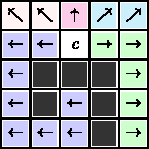
\includegraphics[width=\linewidth]{images/botea-cpd.pdf}
				\caption[Movement information in grid-based CPD.]{Movement-grid for cell $c$ in a grid-based CPD\cite{botea-cpd-2013}.}
				\label{fig:cpd}
			\end{wrapfigure}
			
			The complex part of constructing a CPD is the compression\cite{botea-cpd-2013} of the all-pairs shortest path solution.
			Uncompressed data is usually too large as the space requirement is in $\bigo{n^2}$ or even $\bigo{n^2 \log n}$ for graphs.
			A combination of compression techniques can be used to get sufficient results.
			This includes the encoding of whole areas with the same movement operations, \term*{run-length encoding} (\term*{RLE}) and the use of default values to reduce the number of explicitly stored values\cite{botea-cpd-2013}.
			Compared to uncompressed data, a compression factor of 950 was achieved for a road network.
	
\section{Geometric routing}
\label{sec:geometric-routing}

	Finding paths in a geometric domain, also called the \term{euclidean shortest path} problem, is the process of determining shortest paths without a graph but through open spaces avoiding obstacles.
	There are two main strategies for finding Euclidean shortest paths:
	Generating edges for graph-based routing or creating a shortest paths map, a structure similar to CPDs.
	
	\subsection{Visibility graphs}
	\label{subsec:visibility-graph}
	
		The first mechanism uses a standard graph-based shortest path algorithm, but the edges in the graph are generated using one of multiple possible approaches.
		One approach creates a so-called \term{visibility graph}, which is a normal graph with edges between vertices that are visible to each other.
		Or in other words, for any two $u, v \in V$ an edge $(u, v) \in E$ exists if and only if no obstacle intersects with this edge.
		A visibility graph might become very large, the worst-case regarding the size is a complete graph with $\bigo{|V|^2}$ many edges.
		
		Alternatives to the visibility graph generation are based on Voronoi diagrams or skeletonization methods.
		However, routing results on such graphs are not necessarily optimal\cite{graser-osm-open-spaces}, since a straight edge between visible vertices is the shortest possible connection.
		
		Source and destination locations must be part of the graph and can be connected with the same algorithm used to create the graph itself.
	
	\subsection{Continuous Dijkstra paradigm}
	\label{subsec:continuous-dijkstra}
	
		The second strategy, the \term{continuous Dijkstra paradigm}, creates a map of regions, similar to CPDs, starting from a source vertex $s$.
		Regions are characterized by the fact that all vertices within a region have the same predecessor on the shortest path from $s$.
		Following back the predecessors yields the shortest path from $s$ to a given location.
		This map can also be seen as a tree with root $s$ and each region as a node, which might remind one of Dijkstra's algorithm giving this approach its name\cite{mitchell-discrete-geodesic}.
		
		To precisely determine these regions, so-called \term[wavefront]{wavefronts} propagating through open spaces are used.
		A well-fitting analogy for this approach is the propagation of water waves traveling through a 2D space, folding around obstacles, colliding with each other and finally reaching the destination location.
		Collisions between wavefronts and obstacles as well as collisions between two wavefronts determine the regions' boundaries with the source of the wavefront as its predecessor.
		After detecting such a collision, the angular region of the wavefront is adjusted depending on the type of collision.
		The fundamental difficulty of this approach is the efficient detection and handling of collisions.
		Efficient algorithms are presented in \Cref{subsec:related-work-geometric-routing}.

\section{Agent-based systems and simulations}

	Simulating complex systems with numerous autonomous individuals is difficult, but using so-called \term[agent]{agents} with independent behavior and decision-making breaks down this complexity\cite{macal-introductory-tutorial}.
	Interactions between two agents and between agents and the environment are essential to this.
	
	Modeling agents can be arbitrarily complex because agents make decisions independently without any central controlling unit.
	More sophisticated agents may have a specific goal, can adapt to the environment and thus must be able to memorize and plan things.
	
	Agents usually model humans but can represent non-living things like companies or cars.
	Many simulations use pedestrians (or generally humans) as agents to better understand or utilize human behavior but other scenarios and types of agents are possible as well\cite{macal-introductory-tutorial}.

	Studying pedestrians requires a spatial environment and algorithms finding optimal paths\cite{kneidl-borrmann-hartmann-navigation,gloor-hybrid-pedestrian-routing,teknomo-millonig-routing}.
	This includes \hyperref[sec:graph-routing]{graph-based routing} but may utilize \hyperref[sec:geometric-routing]{geometric routing} as well\cite{kneidl-borrmann-hartmann-navigation}.
	In this thesis, these two concepts are combined to enhance the pathfinding component of agent-based simulations.
	
	\subsection{The MARS framework}
	
		This work aims to enhance agent-based simulations created using the framework \term*{MARS} (Multi-Agent Research and Simulation).
		MARS is a C\#/.NET framework to create and execute agent-based simulations and is developed by the eponymous research group of the Hamburg University of Applied Sciences (HAW) in Hamburg, Germany\footnote{\url{https://www.mars-group.org}}.
		The framework provides components, algorithms and tools to create tick-based simulations with multiple agents, different data layers and numerous static entities populating the environment.
		
		MARS contains several data structures and algorithms specifically for pathfinding, such as a spatial graph and the A* algorithm.
		It also contains numerous spatial indices, mathematical operations and classes to serialize the trajectories of agents.
		 
		This work is based on the MARS framework to be directly usable by simulations and uses the mentioned spatial graph and A* algorithm.
		More details on the design and implementation are given in \Cref{chap:design} and \ref{chap:implementation}.
		
	\chapter{Related work}
	\label{chap:related-work}
	
		% !TEX root = ../thesis.tex
% !TeX spellcheck = en_US

Scientific literature contains related work from many different areas, mostly from geodata, graph construction and networks as well as routing and (pedestrian) path planning.
This section gives an overview about closely related work from these areas.

\section{Graphs and networks}

	% with some assumptions like no dollinear vertices (even though these assumptions are not necessary): Constructing the visibility graph for n-line segments in O(n²) time (Emo Welzl, 1985)
	Constructing a visibility graph is an important part of this thesis.
	The construction of visibility graphs in $\bigo{n^2}$ time and space (with $n$ line segments), under the condition of no collinear coordinates and no intersecting line segments, was presented by Welzl in 1985\cite{welzl-visibility-graph}.
	A few years later, Overmars and Welzl presented two new methods reducing the space complexity to $\bigo{n}$\cite{overmars-weizl-visibility-graph}.
	Their new algorithms are based on Welzls earlier paper and the idea of a rotational sweep through neighboring vertices.
	
	% maybe, they use geom. routing to fill OSM gaps: Automatic extrapolation of missing road network data in OpenStreetMap (Funke, Schirrmeister, Storandt, 2015)

\section{Routing}

	% Shortest paths among obstacles in the plane (Mitchell, 1993)
	Shortly after Welzl and others published their work on visibility graphs, which can be used in combination with Dijkstra to find shortest paths, Mitchell presented a pure geometric method to find euclidean shortest paths around obstacles in the plain in 1993\cite{mitchell-shortest-path}.
	He used wavefronts propagating from the source towards the target vertex.
	Each origin of a wavefront can be traces back to the source giving the shortest path.
	Because this algorithm solves the \hyperref[subsubsec:single-source-shortest-path]{\term*{single-source shortest path} problem} just like the Dijkstra algorithm does on a network, this technique is also called the \term{continuous dijkstra} paradigm.
	
	% An Optimal Algorithm for Euclidean Shortest Paths in the Plane (Hershberger, Suri, 1999)
	Another approach solving the geometric single-source shortest path problem was presented by Hershberger and Suri one year later, in 1997.
	They also use the \term*{continuous dijkstra} paradigm but increase performance by introducing a special quad-tree like structure and smart subdivision of the plain.
	The result is then actually a path map allowing shortest-path request to be processed in only $\bigo{n \log n}$.
	
	% maybe: Efficient algorithms for Euclidean shortest path and visibility problems with polygonal obstacles (Kapoor, Maheshwari, 1988)

\section{Pedestrian path finding}
	
	A special case of the general single-source shortest path problem is pedestrian routing, also called pedestrian shortest-path finding.
	This problem is especially interesting since pedestrians have the maximum degree of flexibility/freedom compared to other traffic participants like bikes or cars.
	Therefore, geometric routing is a good way to find shortest-paths for pedestrians.
	
	Pedestrian path finding is, however, not only relevant for real world users, who want to know how to get from one location to another.
	Such algorithms are also used in (multi) agent simulations of pedestrian behavior.
	Scenarios in such simulations are for example evacuation or crowd behaviors.
	The area of pedestrian path planning and simulations is divided into two strategies: Network and field based path finding\cite[2]{hartmann-geodesic}.
	Work from both strategies will be covered here.
	
	\subsection{Field based navigation}
		
		% online routing: A Navigation Algorithm for Pedestrian Simulation in Dynamic Environments (Teknomo, Millonig, 2007)
		Teknomo and Millonig created a dynamic algorithm which does not pre-compute the path with one of the above mentioned approaches\cite{teknomo-millonig-routing}.
		This is interesting, since the probably most common and naive approach is to pre-compute the route used by an agent within a simulation.
		The term \enquote{dynamic} refers to the fact, that real world pedestrians often only consider the near neighborhood within their path planning.
		Even if a person knows the hole area, dynamic changes (closed doors, construction work, crowds blocking the way) can still occur at any point in time.
		Therefore, such dynamic considerations can be one aspect to make simulations more realistic.
		
		% maybe: pure geometric/geodesic approach with navigation fields: https://iopscience.iop.org/article/10.1088/1367-2630/12/4/043032/pdf
		The above mentioned dynamic routing by Teknomo and Millonig has strong similarities to approaches based on potential fields, like the dynamic path finding from Hartmann, 2010\cite{hartmann-geodesic}.
		He proposed a mechanism using vector fields in a cellular automaton model with hexagonal cells.
		Interestingly, this method can be interpreted as wavefronts, like in Mitchells algorithm described above, propagating through the vector field\cite[4]{hartmann-geodesic}.
			
		% unified pedestrian routing (they use the above navigation field graph generation): A Unified Pedestrian Routing Model for Graph-Based Wayfinding Built on Cognitive Principles (Kielar, et al. 2017)
	
	\subsection{Graph generation for pedestrian navigation}
	
		An alternative to field based approaches are graph based ones, where a graph is constructed and then used in navigation.
		The construction can be based on potential fields but also on the above mentioned \term*[visibility graph]{visibility graphs}.
		
		In fact, Gloor, Stucki and Nagel presented a pedestrian navigation model and a comparison of these two strategies regarding their performance\cite{gloor-hybrid-pedestrian-routing}.
		They developed this model for a pedestrian simulation in the Alps, where a hiking network should be enhanced with additional navigation information.
		Two approaches were presented: A potential field based method, which is used in navigation when needed, and a visibility graph, which is merged into the existing hiking network.
		The visibility graph strategy strongly relates to this thesis.
		For the performance evaluation, they used an evacuation scenario.
		The results showed, that both navigation mechanisms are comparably fast.
		
		A very similar approach, at least with visibility graphs as a base, was chosen by Kneidl, Borrmann and Hartmann to produce a sparse navigation graph\cite[5]{kneidl-borrmann-hartmann-navigation}.
		They chose the construction of a visibility graph over generalized Voronoi diagrams for more realistic edges.
		
		Another interesting paper on enhancing existing navigation graphs, like Gloor, Stucki and Nagel did, was presented in 2016 by Anita Graser by integrating visibility graph edges into the existing OSM data model\cite{graser-osm-open-spaces}.
		Again, the visibility graph was the preferred method of producing edges.
		Considered and discussed alternatives here were two skeletonization methods and a simple grid places over open spaces.
	
	\chapter{Design}
	\label{chap:design}
	
		% !TEX root = ../thesis.tex
% !TeX spellcheck = en_US

This chapter covers the design of the implemented hybrid routing algorithm.
First, the overall context is presenting specifically the requirements and constrains of the algorithm.
Second, details on the decisions regarding the routing strategy and general design are presented.
Finally, an overview of the separate components is given as well as a description on the deployment of this algorithm.

\section{Requirements and constrains}

	% Used by agents for wayfinding
	The primary goal of the hybrid routing algorithm is to provide a path planning algorithm that is integrated into the MARS framework and offers more accurate paths compared to common graph based algorithms on road datasets, thus, enhancing agent based simulations.
	Such a major goal implies several constrains on the architecture and design of the software.
	
	\subsection{Requirements}
	
		Functional requirements of the resulting software can be formulated quite easily, since this is not a large commercial product.
		The hybrid routing algorithm should determine an optimal path between two locations following ways and traversing open spaces while avoiding obstacles.
		A configurable weight function should be used to assign a weight to each edge in order to find the path with the minimum weight.
		Processing of geospatial data must consider existing road network data as well as obstacles, which are features that will be avoided on paths traversing open spaces.
		It must be possible for the shortest path to alternate between segments following roads and open spaces.
		
		More complex and time consuming are the quality requirements.
		Because this is not part of a commercial software development, these requirements are not part of any tender and were not even formulated.
		Nonetheless, they exist and consist of the following aspects.
	
		The largest quality requirement in terms of effort is performance.
		It affects large parts of the software architecture since the resulting algorithm, despite its complexity, should ideally have a negligible impact on the overall performance of a simulation compared to current graph based routing approaches.
		Routing algorithms and engines often consist of two steps: preprocessing and answering routing queries.
		In order to create fluent and fast simulations, the performance of answering numerous routing requests must be as good as possible.
		The time needed for preprocessing is of less importance.
		
		A rather obvious requirement is the correctness of resulting routes.
		Answers of routing queries must return the shortest route according to a given weight function.
%		Even when using an approximation algorithm to determine shortest paths, the results can be checked against all other possible paths to verify the optimality of the resulting path.
		
		Another quality requirement is the closeness of the resulting routes to real pedestrian behavior.
		Unfortunately, this can hardly be measured without having extensive data of real world pedestrians in real world locations.
		Ideally, the trajectory of a calculated route should be identical to a real world pedestrian trajectory.
		It should at least make sense to an observer without additional knowledge of the real world location.
		The coordinates of waypoint on the calculated and on real trajectories must not be exactly the same, since real pedestrian behavior is not part of the shortest path calculations but is instead a task for realistic agent modeling.
		Such behavior includes for example a typical minimum distance kept to obstacles or a minimum radius of walked curves.

		Next to the domain specific requirement, the overall code itself should of course be well documented and tested.
	
	\subsection{Constrains}
	\label{subsec:constrains}
		
		% Well integrated into MARS and NTS, no new dependencies
		One major constraint is the integration of final algorithm into the \term*{MARS} framework to make the use as easy as possible and to centralize the code base for better maintenance.
		This means the programming language will be C\# and additionally, because MARS uses the geospatial framework \term{NetTopologySuite} (\term*{NTS}) as basis for all major geospatial operations, this algorithm will be based on NTS.
		
		The planned integration into another code base affects the management of dependencies.
		On the one hand, the amount newly introduced dependencies should be kept to a minimum.
		On the other hand, using only libraries on which MARS depends as well is not always possible due to version mismatches.
		However, the latter case can be avoided and should disappear with future dependency updates.
	
\section{Combination of routing algorithms}
\label{sec:combining-routing-algorithms}

	This section describes the core aspect of this thesis:
	The decision of a strategy to combine graph and geometric based routing algorithms.
	A decision on this \enquote{merge} strategy to be implemented is crucial to the design and architecture of the application.
	
	In the following, four approaches are discussed of which the last is considered to be the most promising, which was therefore chosen to be implemented.
% STIMMT NICHT:	The first three are using any normal graph based routing algorithm, like A* or Dijkstra, in combination with the geometric continuous Dijkstra paradigm.
%	Only the last and further pursued approach uses visibility graphs for routing.
	
	% Ad-hoc creation of edges by stopping A* and continuing with wavefront algorithm
	\subsection{Approach candidate 1: Ad hoc generation of edges}
	
		The idea of an ad hoc generation of edges is the following:
		Whenever the graph routing algorithm reaches a road junction, it's paused and the continuous Dijkstra algorithm is started.
		No destination vertex is defined, which means the geometric routing will be stopped after the furthest wavelet reached a certain distance.
		The continuous Dijkstra approach actually creates a shortest path map, so the shortest paths to all reached vertices are calculated.
		All shortest path edges are then added to the graph for the paused graph based routing algorithm.
		
		A real world example for this approach would be a pedestrian walking down a road, stopping at a junction to decide where to go and choosing the option to cross a park for a shortcut before continuing to follow the roads again.
		Doing the shortcut was not planned but an ad hoc decision, just as the algorithm would do.
		
		The advantage of this approach is the realistic behavior of pedestrians not planning the route in beforehand.
		In fact Teknomo and Millonig introduced a routing mechanism for agent based simulations with the assumption of little to no apriori knowledge of agents about their environment \cite{teknomo-millonig-routing}.
		This approach would therefore implement their assumptions on agents behaviors.
		
		One disadvantage is a relatively high complexity since no standard algorithm from frequently used software frameworks support a pause functionality, so any routing algorithm has to be manually adjusted or implemented from scratch.
		
		Also this approach will likely cause performance issues.
		When using Dijkstra as graph based routing algorithm, $\bigo{|V|}$ many vertices are visited, which leads to $\bigo{|V|}$ routing requests using the geometric continuous Dijkstra algorithm.
%		Because a simple caching of the shortest path map is not possible, at least not without a smart and complex caching strategy, this decreases the runtime of the whole routing process significantly.
		Even when using the continuous Dijkstra approach from Hershberger and Suri \cite{hershberger-suri} with only $\bigo{n \log n}$ time requirement, the number $n$ of vertices in obstacles is expected to be much higher than the size of $V$ resulting in a somehow quadratic runtime.
		Caching the shortest path map using a \term*{CPD} (see \cref{subsubsec:cpd}) would be possible but would also increase complexity during query time and reduce performance during preprocessing time.
		Storing precomputed edges in a simple map would reduce complexity, still increase query time but also still reduce precomputation time.
		
		The ad hoc idea of this approach yields no significant advantage compared to a preprocessing.
		Therefore, this approach was not further pursued.
		
%		Another aspect against this approach is the fact that an ad hoc generation of edges will probably not change the resulting shortest path in comparison to a precomputation of these edges.
%		An argumentation for the correctness of this hypothesis can be sketched as follows.
		
%		Assume that the ad hoc generation starts at each road junction vertex $j$ and stops when a certain condition is fulfilled (for example only generating paths of a certain length).
%		When the graph routing algorithm reaches an unvisited junction vertex $j$ from some other vertex $v$, it either used a road edge or preprocessed edge to get there. Therefore, the following two cases exist:
%		\begin{itemize}
%			\item In case a preprocessed edge was used, then the shortest path from $v$ to $j$ would be identical when using a completely preprocessed graph containing this exact edge $(v, j)$.
%			\item In case a road edge was used to get to $j$, then there are two sub-cases.
%			\begin{itemize}
%				\item In case the road edge was in deed the optimal path to $j$, it would have been used in a preprocessed graph as well.
%				\item In case the road edge was not the optimal path, then the ad hoc generation stopped before reaching $j$ (due to the distance or any other stopping condition) and the edge $(v, j)$ was never added.
%			\end{itemize}
%		\end{itemize}
%		Even though, this is not a formal proof, generating a preprocessed graph and using a normal routing algorithm is probably as least as good as using the ad hoc generation approach.
	
	% Concurrent routing: Use A* and wavefront in parallel and merge the results
	\subsection{Approach candidate 2: Concurrent routing}
	
		A different approach would be two concurrent routing queries, one on the normal road graph and one using a visibility or otherwise generated graph.
		Having the two shortest paths, they could be merged into one path, which results in segments with alternating source graph.
		To merge them, first the intersection points need to be determined and then the better segments have to be chosen based on a weight function.
		
		The most prominent advantage is the simplicity of the routing requests, since known routing algorithms could be used.
		Therefore, it would be rather simple to implement and speed up techniques could be used.
		
		However, there are two major disadvantages.
		First, it is uncertain that the two paths are actually intersecting at any point.
		Second, even if they are intersecting, too few intersections on a long route result in suboptimal paths, because the longer a segment gets, the less accurate the weighting becomes.
		Only if the two routes are intersecting frequently enough, the selection of segments based on the weight function could actually result in good routes.
	
	% Concurrent routing for segments (e.g. start new routing calls every 100m)
	\subsection{Approach candidate 3: Concurrent routing on smaller segments}
	
		This approach is very similar to the one above, but it tries to fix the uncertainty of intersections between the two resulting paths.
		Multiple ways are conceivable to ensure that there are enough intersections or to otherwise guarantee that segments are small enough to be merged.
		
		One way is to stop the routing after a certain distance stopping at the next available vertex.
		After stopping for the first time, there are two such vertices, one where the road network based routing stopped and one where the routing on the generated graph stopped.
		From each vertex, two new routing queries start and stop again after a certain distance.
		This continues until one query reaches the destination.
		On the one hand, this would guarantee small enough segments for later merging, on the other hand, this results in $\bigo{2^n}$ many routing queries.
		Even though each query is short, this approach would probably, even with the help of heuristics or other helping mechanisms, not scale very well.
		
		A different approach to obtain smaller segments would be to first get the shortest path on the road graph.
		Having this path, it is split up into $n$ segments of certain length connecting the vertices $v_0, v_1, ..., v_n$ with $v_n$ being the destination.
		In a next step, shortest paths from each vertex to following vertices are calculates.
		Meaning from $v_i$ paths to $v_{i+1}, v_{i+2}, ..., v_n$ are determined, which unfortunately results in $O(n^2)$ many routing queries.
		Finally, all these paths on the generated graph can be merged together with the query result of the road graph to form a new intermediate graph..
		Finally, one last routing query on this intermediate graph is performed to get the final optimal routing result by using a weight function analogous to the previous approach.
		Instead of an intermediate graph, other combinatorial approaches can be used as well since the shortest path problem can be solved using linear programming \cite{handler-zang-lp-duality}.
		
		There are probably more possible ways to ensure a sufficient amount of segments or intersections, however, this idea was not further pursued.
		
		Unfortunately, both approaches have a worse time complexity than any popular routing algorithms including pure geometric routing.
		Even though the second idea might work well for appropriate segments lengths, the complexity and definite time overhead make it an unfavorable choice.
	
	% Merge of networks
	\subsection{Approach candidate 4: Merge an existing network with a visibility graph}
	
		Previous approach candidates tried to first calculate shortest paths and then merge their results.
		This last approach, which is the currently used one, first merges a generated visibility graph with an existing road graph.
		The actual merge operation is very simple:
		Whenever a road edge and a visibility edge intersect, split the edges, create a new vertex at the intersection point and connect the split edges accordingly.
		
		Even though, this approach is simple and still fast, the main disadvantage is the graph size.
		A visibility graph is large and in most cases it will contain many more edges than the road graph, which negatively affects the routing performance.
		
		Another disadvantage is the time complexity of the merge operation.
		All edges have to be considered and, depending on the number of intersections, edges might be processed multiple times (e.g. one visibility edge might intersect with all road edges).
		This leads to at most $|E_R| \cdot |E_V|$ many merge operations for the routing graph edges $E_R$ and visibility edges $E_V$.
		Complete graphs have the highest number of edges and therefore the highest number of intersections, which gives the upper bound of $\bigo{|E|^2}$ for the merge operation given all edges $E$.
		Fortunately, road networks are very sparse and often have a node degree between three and six \cite{zhao-analysis-osm-bejing}\cite{boeing-osmnx}, resulting in a probably much better runtime behavior in practice.
		\todo[inline]{Maybe analyze this myself for e.g. Germany?}
		\todo[inline]{Link to possible optimizations discussed in later chapters}
		
		Despite the disadvantages of this approach, I considered the advantages to be more important.
		As already mentioned, this strategy is not only simple and fast, compared to some time complexities mentioned previously, but it also allows the use of speed up methods for routing queries.
		Moreover, the resulting path is definitely optimal, based on the given weight function, and no complex postprocessing is needed.
		
		Taken all aspects into account, this strategy seemed to be the simplest and most promising with the least disadvantages.
		It was therefore chosen to be implemented.

\section{Design decisions}
\label{sec:design-decisions}

	With the choice of the merge strategy being the approach of combining two different routing algorithms, several design decisions were made.
	Some decisions did not influence the overall architecture and were just made to enhance performance or simplify the implementation, this section only covers fundamental decisions relevant for the overall architecture.
	\Cref{chap:implementation} covers those decisions that are independent of the overall architecture.
	
	In this work I implemented the visibility graph without the use of algorithms presented in the according \hyperref[subsec:related-work:visibility-graph]{related work section}.
	None of the existing approach would have been easy to implement without problems.
	Details on these problems and the exact reasons that led to the decision of a custom implementation are presented in this section.
	
	\subsection{Requirements and considerations for the visibility graph creation}
	
		One key requirement for the visibility graph creation is the ability to work in arbitrary obstacles, which primarily includes the fundamental point, linestring and polygon geometries.
		To work with arbitrary real world datasets, assumptions about the collinearity, position of obstacles and intersections between them cannot be made.
		
		An important special case arises for linestring obstacles consisting of more than two points.
		Simply determining visibility edges to and from both sides of the linestring would result in shortest paths leading right through it.
		Of course, this is the opposite of the desired behavior of a shortest path leading \emph{around} the linestring.
		The same situation would arise with obstacles, including polygonal ones, touching in a single node.
		
		Since the visibility graph is solely used to determine shortest paths, some assumptions and optimizations can still be made.
		However, these considerations are not relevant for the overall architecture and are therefore covered in \cref{sec:visibility-graph-creation}.
		
		A core aspect of the routing algorithm is the reachability of arbitrary locations not located on the graph.
		Adding visibility edges after the complete graph has been created must therefore be possible.
		Implementing this is necessary regardless of the chosen algorithm for the visibility graph creation.
		
		One very important reason why no highly optimized approach was chosen and also why only a limited amount of effort went into the optimization of my own approach is the fact that generating the graph is separated from its use.
		Far more significant is the routing behavior itself as it directly affects the simulation time.
		Creating the graph in a preprocessing step has, especially when persisting the graph for multiple uses, no direct effect on the simulation.
		
		All these requirements and considerations, including problems and efforts outlined below, lead to the decision of implementing a simple graph generation approach with some easy but effective optimizations.
	
	\subsection{Suitability of existing approaches}

		The largest and most influential design decision was the decision against an approach from the literature as presented in \cref{subsec:related-work:visibility-graph}.
		Several approaches from the literature have either restrictions on the geometric structures or assume that a certain preprocessing of the data was already performed.
		
		The approach by Welzl \cite{welzl-visibility-graph}, for example, explicitly assumes that there are not collinear vertices, i.e. at least three vertices forming a straight line.
		It may seem unlikely at first that collinear vertices occur in real world datasets, but in fact, at least in OpenStreetMap, it is very common to align touching buildings and other straight obstacles like walls.
		
		An optimization of Welzls approach, by Overmars and Welzl \cite{overmars-weizl-visibility-graph}, only works on non-intersecting line segments.
		Real world data is unfortunately too diverse to fulfill this criterion as polygons, longer linestrings and other more complex data structures exist.
		Preprocessing the data, i.e. cutting all geometries into such non-intersecting line segments, would cause new special cases to solve.
		For example, cutting a polygon into line segments would add visibility edges within the former polygon, which needs to be avoided e.g. by storing metadata about the relations of these line segment to each other.
		Handling all those special cases, preventing unwanted edges and still using the approach by Overmars and Welzl would be possible but would also increase the complexity of their approach.
		
		Another approach with the limitation of no collinear vertices was the plain-sweep algorithm by Ghosh and Mount \cite{ghosh-output-sensitive-vgraph}.
		Next to the limitation on collinear vertices, they assume x-coordinates to be unique, which, even though it is very likely fulfilled in real world datasets, would need to be handled as well.
		
		Kapoor and Maheshwari presented a visibility graph creation as well \cite{kapoor-shortest-path-vgraph} but assumed a triangulation of the open space between the obstacles.
		Such a triangulation can be done quite fast, algorithms with time complexities of $\bigo{n \log{n}}$ and better are known \cite[58-60]{de-berg-computational-geometry}, but libraries such as MARS or the NetTopologySuite do not implement this.
		They only provide triangulation methods for polygons but not for the space between them.
		Implementing an algorithm for this task would be needed in addition to the visibility graph creation itself.
		
		Probably all approaches from the literature would work but preprocessing, restrictions on the input data or adjustments to the approaches would be necessary.
		Since this work focuses more on the overall concept of a hybrid routing algorithm, the choice on the graph generation algorithm was of less importance.
		Therefore, the implementation is much simpler and independent of the above mentioned approaches.
	
\section{Components}
\label{sec:components}

	% Generator classes, HybridVisibilityGrahp class and helper functions
	Since this works resides in a rather technical and algorithmically oriented context, there are not many separate components needed to implement a hybrid routing approach.
	One component if the so called \term{hybrid visibility graph}, which is the final output graph consisting of the merged road and visibility edges.
	These edges are created by the according generator component.
	Finally, the merging and creation of the hybrid visibility graph takes place in a third component.
	
	\begin{figure}[h]
		\begin{figcenter}
			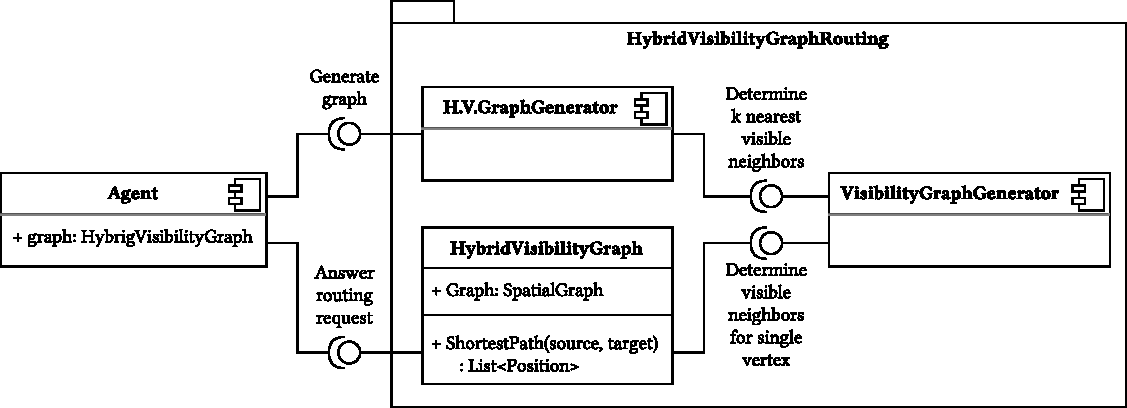
\includegraphics[width=\textwidth]{images/components.pdf}
		\end{figcenter}
		\caption{The components and usages of interfaces of the resulting implementation.}
		\label{fig:components}
	\end{figure}
	
	The first step for a consumer of the system, e.g. an agent based simulation, is to generate the hybrid visibility graph.
	Hence, the \texttt{HybridVisibilityGraphGenerator} (abbreviated as \enquote{H.V.GraphGenerator} in \cref{fig:components}) presents a public interface for this task.
	The result of the graph generation is an instance of the \texttt{HybridVisibilityGraph} class offering public methods to answer shortest path requests, such as the \texttt{ShortestPath} method returning a list of positions (i.e. coordinates) representing the shortest path between two input coordinates.
%	More details on the graph generation can be found in \cref{sec:graph-generation}.
	
	For convenience and due to required preparations, routing queries are put to the hybrid visibility graph.
	To fulfill the overall concept of this work, it must be possible to start and end at arbitrary locations, thus, there is no guarantee that the source and destination locations of the query are on any vertex in the graph.
	Therefore, the hybrid visibility graph has to temporarily connect these locations to the graph.
	This is done by determining all visible neighbors of the source and destination locations and then merging the resulting edges to the underlying graph.
	To perform this task, the hybrid visibility graph uses the interface of the \texttt{VisibilityGraphGenerator} to determine visibility neighbors of a single vertex.
	\Cref{sec:answering-queries} covers the process of answering routing queries in more details, including the clean up step that is performed after the shortest path has been found.

\section{Deployment view}

	% published in MARS
	\todo{Publishing in MARS}


	
	\chapter{Implementation}
	\label{chap:implementation}
	
		% !TEX root = ../thesis.tex
% !TeX spellcheck = en_US

This section describes more implementation details of the previously described approach.
First, an overview of the algorithm with a short description of used frameworks and technologies is given.
After that, the main sections of this chapter show details of each algorithmic step.

\section{Algorithm overview}

	\subsection{Frameworks and technology}
	
		As mentioned in \cref{subsec:constrains} about the constrains, the used programming language is C\# due to the dependency to the MARS framework.
		The MARS framework is based on the widely used C\# library \term{NetTopologySuite} (\term*{NTS}), which contains numerous data structures, algorithms and helper function to handle and process geospatial data.
		
		The NTS was primarily used for basic data structures like features and geometries.
		Writing data to files is also done using NTS functions to serialize the geospatial data into GeoJSON files.
		
		The \term*{MARS} framework was also used for basic data structures, like the \texttt{Position} class.
		However, higher level structures like quadtrees and mathematical calculations were used as well.
		
		Not all data structures and algorithms already existed to create the hybrid routing graph.
		Most notably, a fast line intersection check was implemented as well as a bin based index structure.
		Several other helper functions and simpler structures, like a separate class for vertices, were added as well.

	\subsection{Early implementation based on the continuous dijkstra paradigm}
	
		An early implementation was not creating a visibility graph but instead it was based on the \term*{continuous dijkstra} paradigm with wavelets propagating through open spaces.
		However, there were two reasons why this first approach was replaced by a visibility graph based algorithm.
		
		The first reason was a bad performance.
		Early stages of the continuous dijsktra approach used a very naive and simple implementation without optimizations mentioned in recent literature on this topic.
		Before investing larger efforts into the implementation of a more complex approach, like the one presented by Hershberger and Suri\cite{hershberger-suri}, a simple preprocessing was introduced and lead to a major performance enhancement.
		This perprocessing determined the visibility between all vertices, which was later used to create events for the collision between wavelets and vertices.
		Such predetermined visibilities are the core of a visibility graph, thus moving to an actual visibility graph based approach was not a big step.
		
		The second reason to actually move towards a visibility graph was the difficulty and the disadvantages of combining the network based routing with the continuous dijkstra algorithm implemented so far, as described in \cref{sec:combining-routing-algorithms}.
		Therefore, the decision fell in favor of implementing and optimizing the creation of a routable visibility graph.
	
	\subsection{Chosen approach and potentially faster known algorithms}

		% Maybe this whole subsection is part of a later discussion?
		Due to the step by step development by turning the former continuous dijkstra preprocessing into a visibility graph generator, the implemented approach does not follow algorithms described in the literature.
		The performance of this implementation, as shown in \todo[inline]{link to chapter}, is still enough for practical use, but a well designed and fast algorithm, like the one presented by Overmars and Welzl \cite{overmars-weizl-visibility-graph} or the one by Ghosh and Mount \cite{ghosh-output-sensitive-vgraph}, would clearly increase performance.
		However, this performance enhancement would only affect the generation of a visibility graph and not the performance of the routing queries.
			
	\subsection{Algorithm steps}
		
		As describes in \cref{sec:components}, the \texttt{HybridVisibilityGraphGenerator} class provides a factory method to create a \texttt{HybridVisibilityGraph} from a given collection of features.
		This factory method consists of the following top level steps.
		\todo[inline]{more?}
		
\section{Visibility graph creation}
		
	\subsection{Step 1: Obstacle filtering and feature preprocessing}
	\label{subsubsec:step-1-preprocessing}
			
			First the features are filtered to get all relevant obstacle features, which are of arbitrary shape.
			For performance reasons, multi-geometries, like \texttt{MultiPolygon} are split up into their separate geometries.
			This is not only unproblematic for \texttt{MultiLineString} but also for \texttt{MultiPolygon} features, since holes in a polygon are not reachable in the first place and unwrapping the \texttt{MultiPolygon} will not change this.
			% TODO Better formulation?
			Another task within this first step is the triangulation of all polygonal shapes.
			The main reason is a better performance for intersection checks, which is an important task of creating a visibility graph.
			
	\subsection{Step 2: Determining $k$ nearest visible neighbors}
			
			After having all preprocessed obstacles, the main task of the visibility graph creation is performed, namely determining all $k$ many visible neighbors.
			Determining all visible neighbors would also be possible, but this parameter is an easy way to increase performance with the downside of not having all possible edges in the final routing graph.
			
			\subsubsection{Overview and terminology}
			
				Before describing the details on determining the $k$ nearest neighbors, there are some terms that need to be defined.
				
				\begin{description}
					\item[\term*{visibility neighbor}] Sometimes also just \emph{visible neighbor} is a vertex $u$ that is visible from the currently processed vertex $v$.
					\item[\term*{obstacle neighbor}] This is a vertex $u$ with an existing edge to or from the currently processed vertex $v$. In other words, $u$ is visible from $v$ but via an existing obstacle edge.
					\item[\term*{shadow area}] This is an angle area that starts at a certain distance, for example \enquote{10° to 20° with a minimum distance of 30 meter}.
				\end{description}
			
				\noindent The performed steps of determining the visible neighbors are the following, more details are given in the section below.
				\begin{enumerate}
					\item Get the obstacle neighbors for each vertex.
					\item For each vertex $v$, determine its visibility neighbors as follows.
					\begin{enumerate}
						\item For each other vertex $u$, do the following:
						\begin{enumerate}
							\item Is $u$ in any shadow area? If so, which means $u$ is not visible, move to the next other vertex. Continue otherwise.
							\item Query all obstacles between $v$ and $u$.
							\item Create and store the shadow area of each such obstacle $o$.
							\item Mark $u$ as visibility neighbors if $u$ is still not in any shadow area and a line segment from $v$ to $u$ intersects with none of the above queries obstacles.
						\end{enumerate}
						\item Sort visibility neighbors into bins based on the obstacle neighbors.
					\end{enumerate}
				\end{enumerate}
			
			\subsubsection{Parameter $k$}
			
				The $k$, however, is not just a single parameter, but rather consists of two separate values:
				The number of bins and the number of maximum neighbors per bin.
				Each bin covers a certain angle area of each vertex, for example for a bin count of 36, each bin would cover a 10° area.
				Without this subdivision of the neighbors, it is possible to only have edges to complex and close objects but no edges to obstacles further away.
				
				An example for this would be a large and open park where the $k$ nearest neighbors are probably all at the side of the park where the currently processed vertex is, even though the far away other side of the park is clearly visibly.
				This subdivision into bins ensure that there will definitely be connections to the other side of the park.
			
			\subsubsection{Determining obstacle neighbors}
				
				Determining the obstacle neighbors is relatively simple and straight forward.
				Each coordinate $c$ of an obstacle $o$ is processed by looking at the previous and next coordinates $c_p$ and $c_n$ on that obstacle, which are the potential neighbors.
				If the line segment $(c, c_p)$, for $c_n$ respectively, does not intersect with any obstacle, it is considered an obstacle neighbor.
				
			\subsubsection{Shadow areas}
			
				Shadow areas are a simple method to quickly determine vertices that are definitely not visible to each other.
				The idea of shadow areas is the following:
				Let $v$ be the currently processed vertex and think of it as a light bulb illuminating its surroundings.
				An obstacle $o$ casts a shadow outwards and everything within this shadow is definitely not visible from $v$.
				
				The distance from which everything within the angle area of the shadow is definitely not visible from $v$, is determined by the two bounding vertices (marked in red in \cref{fig:shadow-area}).
				These bounding vertices determine the angular range and the furthest of these two determines the minimum distance of the shadow area.
				
				Keeping track of these shadow areas for each vertex significantly improves performance.
				\todo[inline]{conrete numbers?}\todo[inline]{Reference to BinIndex below or other used data structure (s. TODO below)}
				% NetworkRoutingPlayground->Jungfernstieg dataset with 7916 vertices: ~7.3s with and 67s without shadow areas -> speed up of factor ~9
				% Hamburg inner city dataset with 67819 vertices: 382s with and ~31000s without shadow areas -> speed up of factor ~81
				
				\begin{figure}[h]
					\begin{center}
						\begin{tikzpicture}
							\def\angle{20}
							\def\boundingVertexDistance{3}
							
							\tikzDot[label=$v$]{(0,1.5)}{v}
							\coordinate (shadow-arc-top)				at ($(v) +( \angle:\boundingVertexDistance)$);
							\coordinate (shadow-arc-bottom)				at ($(v) +(-\angle:\boundingVertexDistance)$);
							\coordinate (shadow-arc-top-end)			at ($(v) +( \angle:5.75)$);
							\coordinate (shadow-arc-bottom-end)			at ($(v) +(-\angle:5.75)$);
							\coordinate (shadow-arc-top-faded-end)		at ($(v) +( \angle:6.5)$);
							\coordinate (shadow-arc-bottom-faded-end)	at ($(v) +(-\angle:6.5)$);
							
							% Gray area
							\filldraw[lightgray] 
								(shadow-arc-bottom) arc [start angle=-\angle, delta angle=2*\angle, radius=\boundingVertexDistance] --
								(shadow-arc-top-end) --
								(shadow-arc-bottom-end) --
								cycle;
							\draw[gray]
								(shadow-arc-bottom-end) --
								(shadow-arc-bottom) arc [start angle=-\angle, delta angle=2*\angle, radius=\boundingVertexDistance] --
								(shadow-arc-top-end);
							
							\draw[dotted] (v) -- (shadow-arc-top);
							\draw[dotted] (v) -- (shadow-arc-bottom);
							
							% Faded gray area
							\filldraw[draw=none,lightgray,path fading=east]
								(shadow-arc-top-faded-end) --
								(shadow-arc-top-end) --
								(shadow-arc-bottom-end) --
								(shadow-arc-bottom-faded-end) --
								cycle;
							\draw[gray,path fading=east] (shadow-arc-top-end) -- (shadow-arc-top-faded-end);
							\draw[gray,path fading=east] (shadow-arc-bottom-end) -- (shadow-arc-bottom-faded-end);
							
							% Obstacle 1
							\tikzDot[red]{(shadow-arc-top)}{o10}
							\tikzDot{(3.5,2)}{o11}
							\tikzDot[red]{($(v) +(-\angle:1.2)$)}{o12}
							\node[above right = 0.5 and 1 of o12] {$o_1$};
							
							% Obstacle 2
							\tikzDot[label=right:$v'$]{(3.5,1.35)}{o20}
							\tikzDot{(3.5,-0.25)}{o21}
							
							% Obstacle 3
							\tikzDot[label=right:$v''$]{(2.1,1.1)}{o30}
							\tikzDot{(2.1,-0.5)}{o31}
							
							\node[darkgray] at (4.65,1.5) {\huge$S$};
							
							\draw (o10) -- (o11) -- (o12) -- (o10);
							\draw (o20) -- node[right] {$o_2$} (o21);
							\draw (o30) -- node[left] {$o_3$} (o31);
						\end{tikzpicture}
					\end{center}
					\caption{Shadow area $S$ cast by obstacle $o_1$ seen from vertex $v$. The vertex $v'$ of obstacle $o_2$ is not visible from $v$ since it lies inside the shadow area. The two red vertices of obstacle $o_1$ are the bounding vertices determining angle range and distance of $S$. Not that $v''$ is not visible from $v$ as well even though it is not inside the shadow area.}
					\label{fig:shadow-area}
				\end{figure}
				
			\subsubsection{BinIndex data structure}
			
				The \texttt{BinIndex} class implements a simple index structure to store and access intervals.
				It contains $n$ many bins of which each covers a certain range and consists of a linked list.
				When an item is added, it is added to each bin intersecting with the range of the item.
				Due to the list as underlying data structure for the bins, queries can be answered in $\bigo{m}$ time for $m$ many items in the index.
				
				The NetTopologySuite offers several indices specifically made for intervals, namely the \texttt{BinTree} and \texttt{SIRtree}, of which the latter one is static and does not allow insertions after the first query was made.
				Even though these two structures are tree based and theoretically offer a logarithmic query complexity compared to the linear complexity of the \texttt{BinIndex}, the simple and list based \texttt{BinIndex} is significantly faster even for larger datasets with tens of thousands of vertices.
				It is thinkable that the logarithmic complexity is useful for huge datasets with millions of vertices, but that has not been tested.
			
			\subsubsection{Intersection checks}
			
				All intersections are checked using own implementations no not rely on the generalized and therefore slower intersection checks of the NetTopologySuite.
				In fact, there are two types of intersection checks implemented:
				One check for intersection between two arbitrary line segments and one checks if a point lies within a triangle.
				This triangle check is used for closed obstacles, which got triangulated during \hyperref[subsubsec:step-1-preprocessing]{preprocessing}.
				
				The line segment intersection check uses a cross product based approach described in \emph{Introduction to algorithms} by Thomas H Cormen et al \cite[1018]{cormen-introduction-to-alg}.
				
				Checking if a point lies inside a triangle is done by a barycentric collision check.
				This method creates a barycentric coordinate system where each coordinate consists of three values $\lambda_1$, $\lambda_2$ and $\lambda_3$ for each corner vertex of the triangle.
				Due to the properties of this coordinate system, a point $p$ is inside the triangle when the condition $0 < \lambda_i < 1$ hold for each of the three values.
				Even though it sounds complex to create a whole coordinate system for a single collision check, this method only uses a few basic arithmetic operations and is therefore very fast.
			
			\subsubsection{Sort resulting visibility neighbors into bins}
			
				A naive approach to create a visibility graph would be to create edges between vertices that see each other.
				This would make routing through line based obstacles possible, which is of course not correct.
				It must therefore be known which visibility relations are between which obstacle neighbors.
				Knowing this enables the graph generation to distinguish between all the edges and results in correct routing results.
				More on this in the \cref{subsec:step-3-graph-creation} below.
				
				Each of the resulting bins of a vertex $v$ covers the area between two adjacent obstacle neighbors.
				All visibility neighbors are sorted into these bins, which is a simple and easy process.
			
	\subsection{Step 3: Graph creation with visibility edges}
	\label{subsec:step-3-graph-creation}
		
	\subsection{Step 4: Merging a road network into the visibility graph}

\section{Answering shortest path queries}
	
	\chapter{Evaluation}
	\label{chap:evaluation}
	
		\section{Performance \& Correctness}
		
			\subsection{Correctness}
			
			\subsection{Performance}
			
			\subsubsection{Used methods and system}
			
			% Maybe: complexity analysis
			
			\subsubsection{Results}
		
		\section{Quality of routing}
		
			\subsection{Usefulness of routes}
			
			% How realistic are the routes (= can I go there in real life)? If not: Why not?
			
			\subsection{Accuracy of simulations}
		
			% Concrete scenario (parameters/model, what happens), evaluation
	
	\chapter{Conclusion}
	
		\section{Future work}
		
	\printbibliography

	\printindex
	
	\chapter*{Appendix}
	
		% !TEX root = ../thesis.tex
% !TeX spellcheck = en_US

\clearpage
\thispagestyle{empty}
\pagestyle{empty}

\begin{center}
	\Large
	\textbf{Eidesstattliche Erklärung}
\end{center}
\noindent
Hiermit versichere ich an Eides statt, dass ich die vorliegende Arbeit im Masterstudiengang Informatik selbstständig verfasst und keine anderen als die angegebenen Hilfsmittel –- insbesondere keine im Quellenverzeichnis nicht benannten Internet-Quellen –- benutzt habe. Alle Stellen, die wörtlich oder sinngemäß aus Veröffentlichungen entnommen wurden, sind als solche kenntlich gemacht. Ich versichere weiterhin, dass ich die Arbeit vorher nicht in einem anderen Prüfungsverfahren eingereicht habe und die eingereichte schriftliche Fassung der elektronischen Abgabe entspricht.

\vspace*{1cm}
\noindent
\begin{tabularx}{\textwidth}{@{}Xr@{}}
	&
	\begin{tabular}{@{}l@{}}
		\makebox[5cm]{}\\ % \includegraphics[width=5cm]{images/signature}
		\hline
	\end{tabular}
	\\
	\noindent
	Hamburg, den XX.XX.20XX
	&
	\makebox[5cm]{Hauke Stieler}
\end{tabularx}

\vspace*{3cm}

\begin{center}
	\Large
	\textbf{Veröffentlichung}
\end{center}
\noindent
Ich stimme der Einstellung der Arbeit in die Bibliothek des Fachbereichs Informatik zu.

\vspace*{1cm}
\noindent
\begin{tabularx}{\textwidth}{@{}Xr@{}}
	&
	\begin{tabular}{@{}l@{}}
		\makebox[5cm]{}\\ % \includegraphics[width=5cm]{images/signature}
		\hline
	\end{tabular}
	\\
	\noindent
	Hamburg, den XX.XX.20XX
	&
	\makebox[5cm]{Hauke Stieler}
\end{tabularx}
\end{document}